\header{
    \headtitle{Qu'on apporte} \label{qu-on-apporte}
    %
    \insertComment{Parue en 1696 dans le chansonier dit de Maurepas sous le titre "L'histoire profane".}{}
}

\enluminure{4}{\href{https://www.youtube.com/watch?v=8NPsvxMdVlg}{L}}{e père} Adam, trois jours avant la faute,
\\Au Paradis ronflait comme un cochon
\\Pour le punir, Dieu lui prit une côte,
\\Souffla dessus et fit le premier...
\\\\\textbf{Refrain (en "on") :}
\\Trim, troum, tram, laridondaine,
\\Trim, troum, tram, laridondon.
\\Souffla dessus et fit le premier...
\\Qu'on nous verse à boire (ter)
\\Du bon vin.
\\\\Ce qui séduit notre première mère,
\\Ce ne fut point ni l'arbre ni le fruit;
\\Le fin serpent, n'aurait pas su lui plaire,
\\S'il n'avait pris la forme d'un gros...
\\\\\textbf{Refrain (en "i") :}
\\Trim, troum, tram, laridondaine,
\\Trim, troum, tram, laridondon.
\\S'il n'avait pris la forme d'un gros...
\\Vite, vite à boire (ter)
\\Du bon vin
\\\\Pourquoi Enée a-t-il quitté Carthage?
\\Pourquoi Enée a-t-il quitté Didon?
\\C'est qu'il voyait, debout sur le rivage,
\\Des femm's troyenn's qui se lissaient le...
\\\\Comment Noé repeupla-t-il la terre
\\Avec sa femm' travaillant jour et nuit?
\\Chacun prétend que c'est par la prière,
\\Mais moi je dis que c'est à coup de...

\breakpage
Les imbécil's, ainsi que les vicaires,
\\Auraient voulu supprimer ma chanson
\\Aucun d'entr'eux ne serait sur la terre
\\Si leur maman n'avait prêté son...

\bigskip
\bigskip
\begin{center}
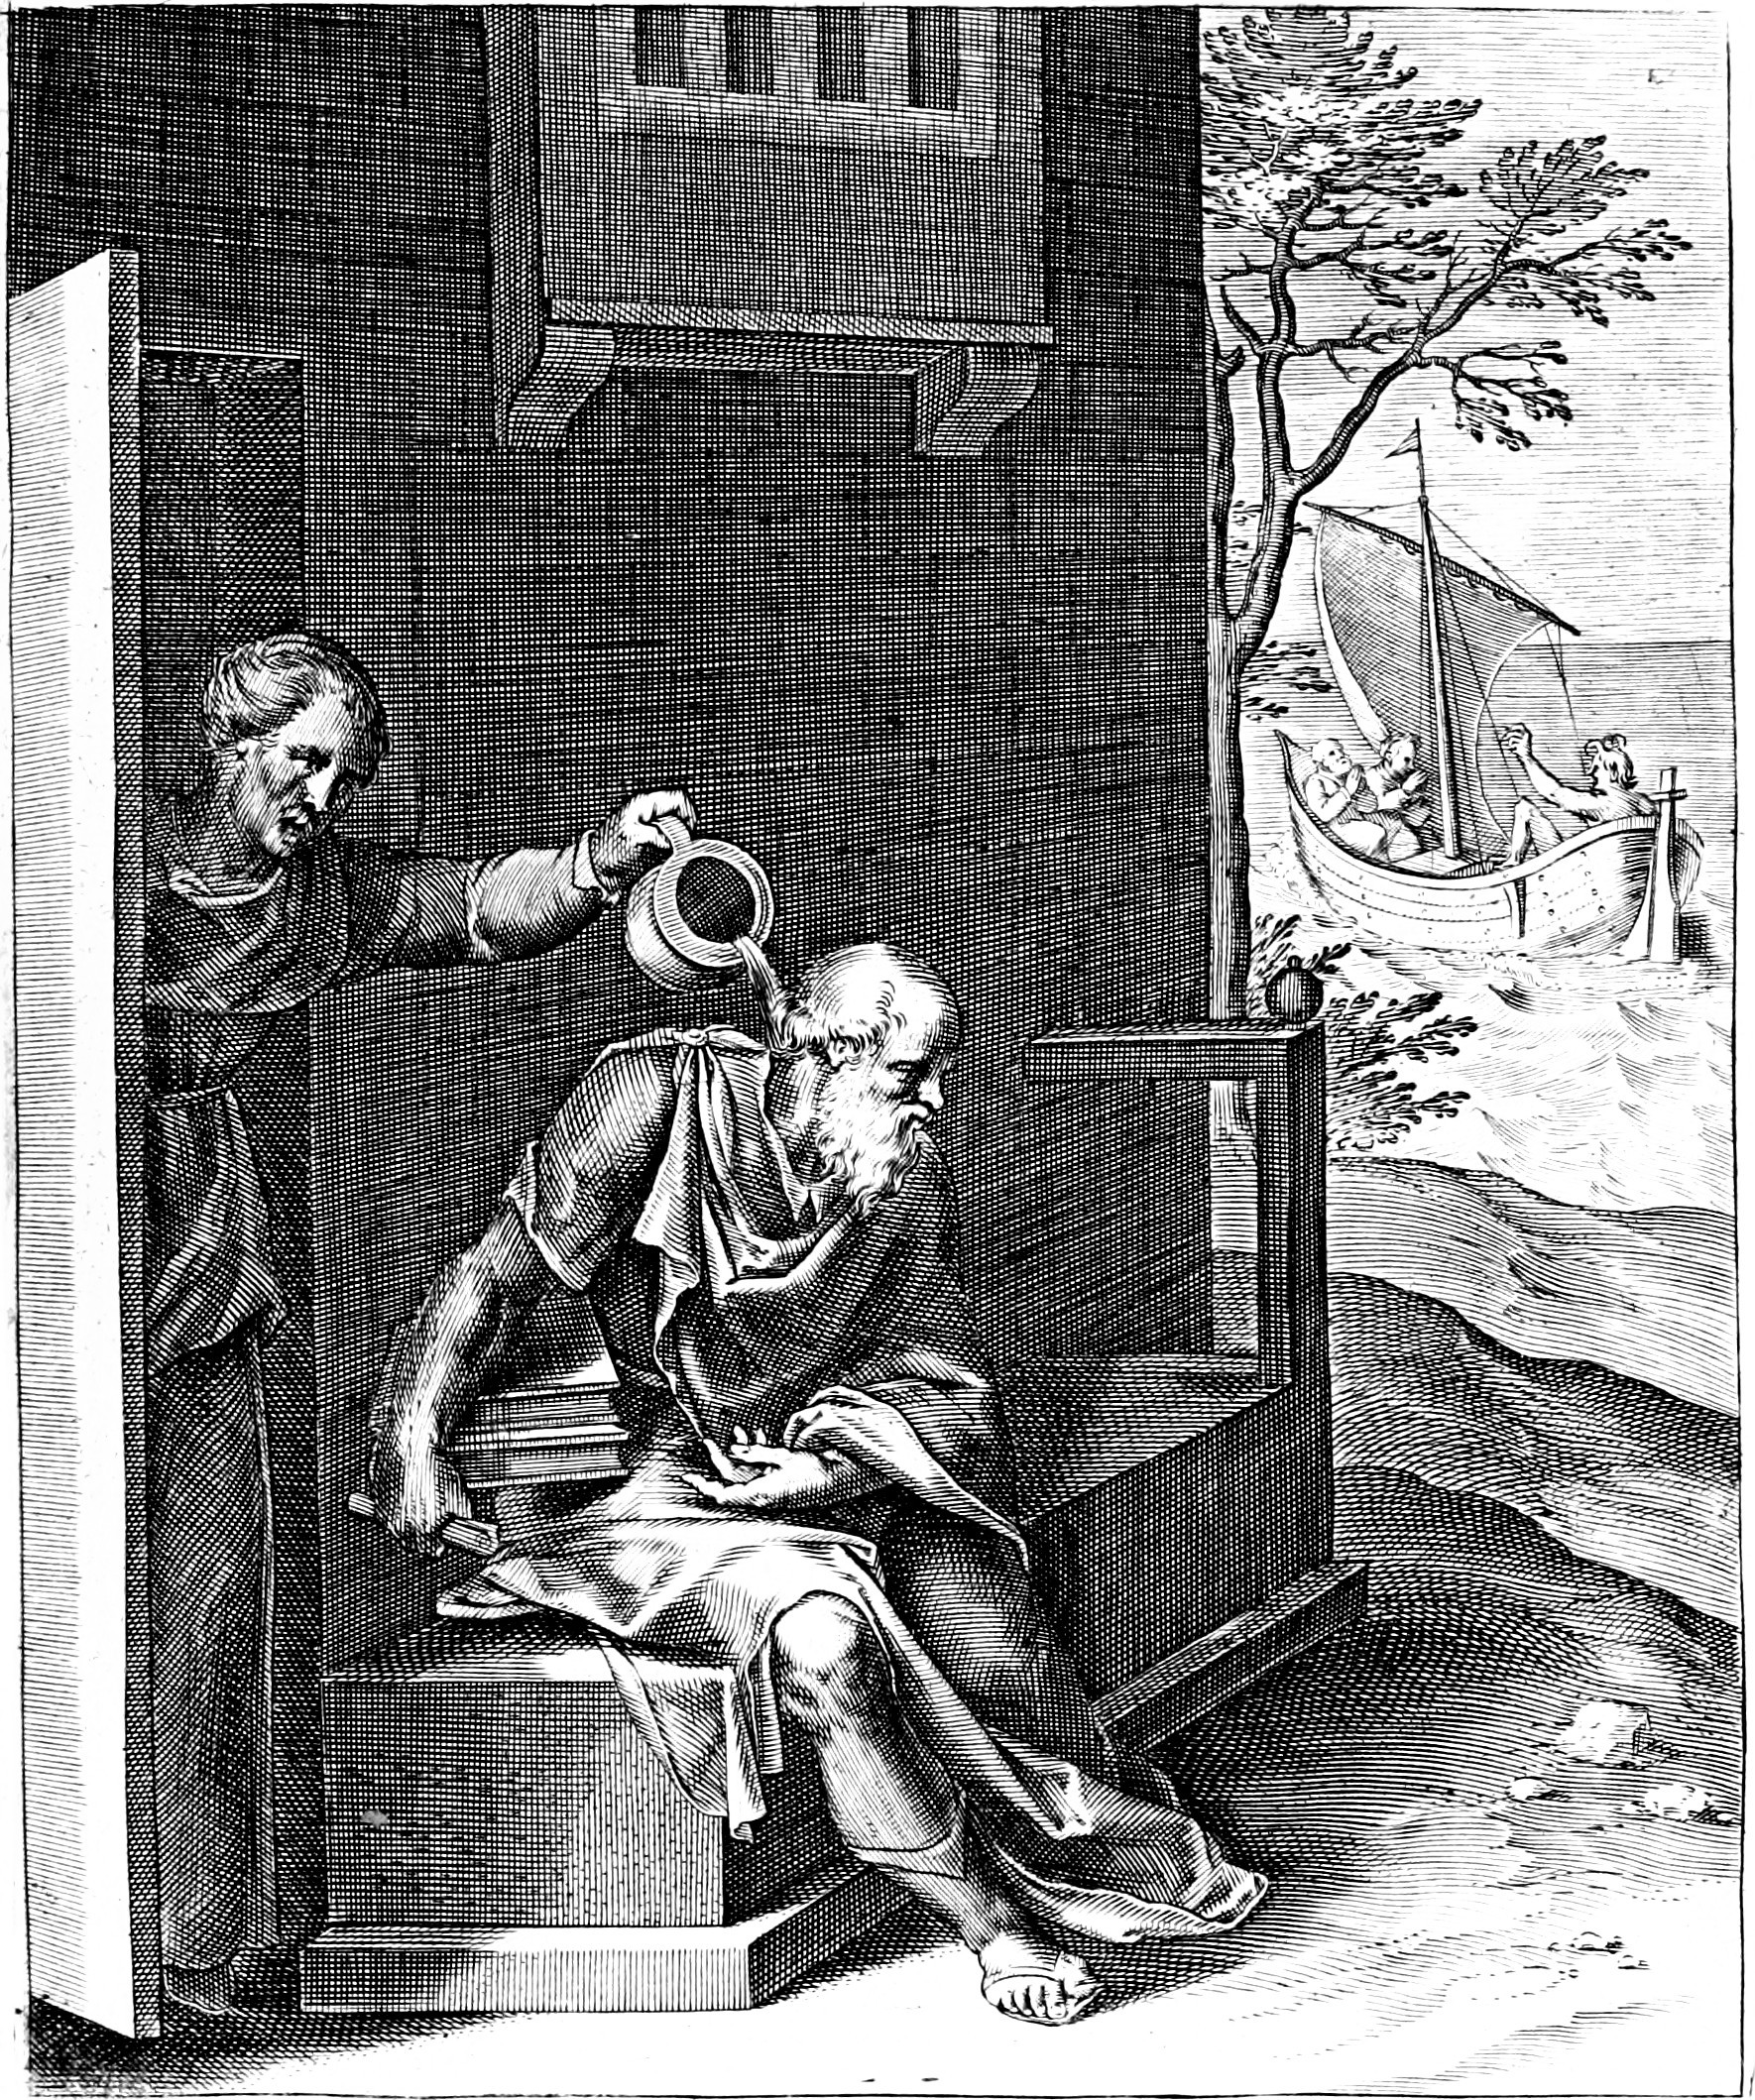
\includegraphics[width=1\textwidth]{images/brev44.png}
\end{center}

\breakpage